

\subsection{Sprint 1}

		\subsubsection{Sprint Planning  | 27 février 2024}
		\begin{enumerate}
			\item Liste de l’ensemble des demandes du client.
			\item Cadrage initial du projet et définition des objectifs; pour se faire : réflexion avec l'équipe et le représentant du client pour se familiariser avec le domaine du produit.
		\end{enumerate}
		
		\subsubsection*{Tâches à réaliser}
		\begin{itemize}
			\item Définition des besoins : surveillance, renseignement, reconnaissance.
			\item Schématisation du navires et de ses drones.
			\item Familiarisation avec la doctrine detection passive.
			\item Prise en compte de la dimension distribution serveur/client pour simuler les échanges entre les systèmes.
			\item Prototype papier d’une base de données pour contenir les rapports de détection, les caractéristiques des drones et l’état des missions.
		\end{itemize}
		
		\subsubsection{Daily Scrum du 12 Mars 2024}
		\subsubsection*{Objectif(s)}
		\begin{itemize}
			\item Liste de l’ensemble des demandes et prise en compte des retours du client.
		\end{itemize}
		
		\subsubsection*{Tâches réalisées}
		\begin{itemize}
			\item Listes des exigences fonctionnelles.
			\item Échange entre le client, son représentant pour éclaircir les zones de flou sur le fonctionnement du système et lever des barrières et des interrogations autour des différents usages du système à travers d’un schéma et d’échanges.
		\end{itemize}



\subsection{Sprint 2}
	
	\subsubsection{Sprint planning | 19 Mars 2024}
	\subsubsection*{Objectif(s)}
	\begin{itemize}
		\item Définitions des objectifs à réaliser entre l’équipe et les représentants du client.
		\item Planification des tâches.
	\end{itemize}
	
	\subsubsection*{Tâches réalisées}
	\begin{itemize}
		\item Réalisation du diagramme de cas d’usage.
		\item Liste des différentes fonctions pour chaque mode du simulateur.
		\item Définition des contraintes du système et de son articulation.
	\end{itemize}
	
	\subsubsection{Sprint Review du 26 mars 2024}
	
	\subsubsection*{Tâches réalisées}
	\begin{itemize}
		\item Réalisation du diagramme statique (objet).
		\item Assimilation des rôles pour la méthode Agile Scrum.
		\item Recherche de développement du code : PyQT ou Tkinter.
	\end{itemize}
	
	\subsubsection{Daily Scrum | 8 Avril 2024}
	\subsubsection*{Objectif(s)}
	\begin{itemize}
		\item Clarification de ce qui a été réalisé, des différentes tâches à finaliser et démarrage d’un cycle extreme programming.
	\end{itemize}
	
	\subsubsection*{Tâches réalisées}
	\begin{itemize}
		\item Échange au tableau sur la conception IHM de notre simulateur.
		\item Développement en binôme : Clément pour la partie serveur et Mattéo pour la maquette de l’interface. Programmation modulaire avec Tkinter en Python3.
		\item Réalisation et reprise des diagrammes UML.
	\end{itemize}
	
	\subsubsection{Sprint Review | 16 Avril 2024}
	\subsubsection*{Objectif(s)}
	\begin{itemize}
		\item Vérification du code et remise en question du développement.
	\end{itemize}
	
	\subsubsection*{Tâches réalisées}
	\begin{itemize}
		\item Ajustement de l’IHM à partir de la maquette.
		\item Échange avec le client pour réviser l’approche client-serveur.
	\end{itemize}
	
	\subsubsection{Sprint Retrospective 1 | 23 Avril 2024}
	\subsubsection*{Objectif(s)}
	\begin{itemize}
		\item Clarification de ce qui a été réalisé.
		\item Reprise des diagrammes UML.
		\item Développement des classes selon le MVC.
	\end{itemize}
	
	\subsubsection{Sprint Retrospective 2 | 29 Avril 2024}
	\subsubsection*{Clarifications}
	\begin{itemize}
		\item Briefing sur ce qui a été réalisé.
		\item Réalisation d'un diagramme de Gantt.
		\item Réalisation d'un diagramme de séquence dynamique
		\item Vérification du code selon le modèle UML.
	\end{itemize}
	
	



\section{Diagramme de Gantt}

\subsection*{29 Avril 2024}
\begin{figure}[H]
	\centering
	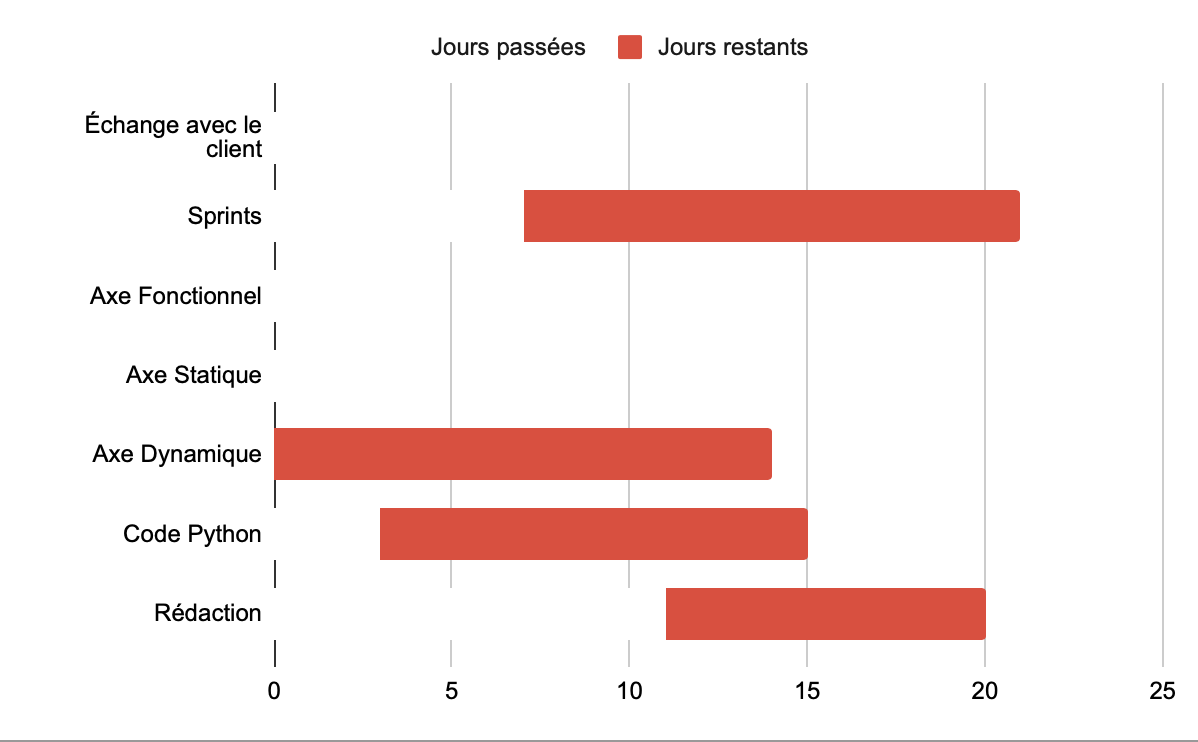
\includegraphics[height=8cm]{img/gantt_290424.png}
	\caption{Diagramme de Gantt le 29 Avril 2024}
\end{figure}

\begin{table}[H]
	\centering
	\caption{Planning du Projet}
	\begin{tabular}{
			>{\columncolor[HTML]{C0C0C0}}l |r|r|r|r|}
		\cline{2-5}
		\cellcolor[HTML]{EFEFEF}                                             & \multicolumn{1}{l|}{\cellcolor[HTML]{C0C0C0}Date de début} & \multicolumn{1}{l|}{\cellcolor[HTML]{C0C0C0}Jours passées} & \multicolumn{1}{l|}{\cellcolor[HTML]{C0C0C0}Jours restants} & \multicolumn{1}{l|}{\cellcolor[HTML]{C0C0C0}TOTAL} \\ \hline
		\multicolumn{1}{|l|}{\cellcolor[HTML]{C0C0C0}Échange avec le client} & 27/02/2024                                                 & 3                                                          & 0                                                           & 01/03/2024                                         \\ \hline
		\multicolumn{1}{|l|}{\cellcolor[HTML]{C0C0C0}Sprints}                & 27/02/2024                                                 & 7                                                          & 14                                                          & 19/03/2024                                         \\ \hline
		\multicolumn{1}{|l|}{\cellcolor[HTML]{C0C0C0}Axe Fonctionnel}        & 23/04/2024                                                 & 4                                                          & 0                                                           & 27/04/2024                                         \\ \hline
		\multicolumn{1}{|l|}{\cellcolor[HTML]{C0C0C0}Axe Statique}           & 19/03/2024                                                 & 3                                                          & 0                                                           & 22/03/2024                                         \\ \hline
		\multicolumn{1}{|l|}{\cellcolor[HTML]{C0C0C0}Axe Dynamique}          & 29/04/2024                                                 & 0                                                          & 14                                                          & 13/05/2024                                         \\ \hline
		\multicolumn{1}{|l|}{\cellcolor[HTML]{C0C0C0}Code Python}            & 29/04/2024                                                 & 3                                                          & 12                                                          & 14/05/2024                                         \\ \hline
		\multicolumn{1}{|l|}{\cellcolor[HTML]{C0C0C0}Rédaction}              & 05/03/2024                                                 & 11                                                         & 9                                                           & 15/05/2024                                         \\ \hline
	\end{tabular}
\end{table}

\subsection*{8 Mai 2024}
\begin{figure}[H]
	\centering
	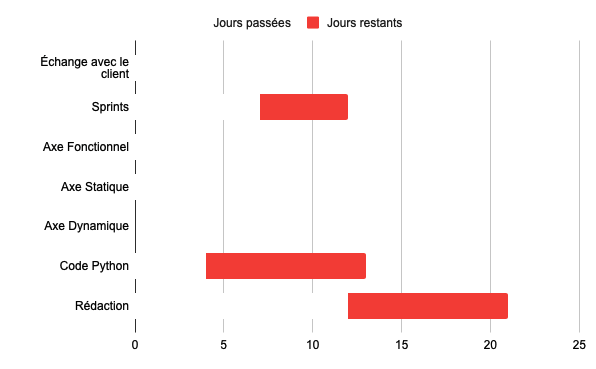
\includegraphics[height=8cm]{img/gantt_08052024.png}
	\caption{Diagramme de Gantt le 8 Mai 2024}
\end{figure}

% Please add the following required packages to your document preamble:
% \usepackage[table,xcdraw]{xcolor}
% Beamer presentation requires \usepackage{colortbl} instead of \usepackage[table,xcdraw]{xcolor}
% Please add the following required packages to your document preamble:
% \usepackage[table,xcdraw]{xcolor}
% Beamer presentation requires \usepackage{colortbl} instead of \usepackage[table,xcdraw]{xcolor}
\begin{table}[H]
	\begin{tabular}{
			>{\columncolor[HTML]{EFEFEF}}l |r|r|r|r|}
		\cline{2-5}
		& \multicolumn{1}{l|}{\cellcolor[HTML]{EFEFEF}Date de début} & \multicolumn{1}{l|}{\cellcolor[HTML]{EFEFEF}Jours passées} & \multicolumn{1}{l|}{\cellcolor[HTML]{EFEFEF}Jours restants} & \multicolumn{1}{l|}{\cellcolor[HTML]{EFEFEF}TOTAL} \\ \hline
		\multicolumn{1}{|l|}{\cellcolor[HTML]{EFEFEF}Échange avec le client} & 27/02/2024                                                 & 4                                                          & 0                                                           & 01/03/2024                                         \\ \hline
		\multicolumn{1}{|l|}{\cellcolor[HTML]{EFEFEF}Sprints}                & 27/02/2024                                                 & 7                                                          & 5                                                           & 19/03/2024                                         \\ \hline
		\multicolumn{1}{|l|}{\cellcolor[HTML]{EFEFEF}Axe Fonctionnel}        & 23/04/2024                                                 & 4                                                          & 0                                                           & 27/04/2024                                         \\ \hline
		\multicolumn{1}{|l|}{\cellcolor[HTML]{EFEFEF}Axe Statique}           & 19/03/2024                                                 & 3                                                          & 0                                                           & 22/03/2024                                         \\ \hline
		\multicolumn{1}{|l|}{\cellcolor[HTML]{EFEFEF}Axe Dynamique}          & 29/04/2024                                                 & 0                                                          & 0                                                           & 13/05/2024                                         \\ \hline
		\multicolumn{1}{|l|}{\cellcolor[HTML]{EFEFEF}Code Python}            & 29/04/2024                                                 & 4                                                          & 9                                                           & 17/05/2024                                         \\ \hline
		\multicolumn{1}{|l|}{\cellcolor[HTML]{EFEFEF}Rédaction}              & 05/03/2024                                                 & 12                                                         & 9                                                           & 17/05/2024                                         \\ \hline
	\end{tabular}
\end{table}

\subsection*{Bilan de la méthode Agile}
Nous avons pu rectifier le livrable que nous allons fournir en un seul logiciel, en deux logiciels distincts (client et serveur). Ces améliorations ont été discutées lors des échanges, tout comme la création d’une interface graphique pour la partie client alors que nous pensions plutôt à une interaction par commande via un terminal.  
